\documentclass[12pt, oneside]{article}
\usepackage[letterpaper, margin=1in, headsep=0.5in, left=0.3in, right=2.5in]{geometry}
\usepackage[english]{babel}
\usepackage[utf8]{inputenc}
\usepackage{amsmath}
\usepackage{amsfonts}
\usepackage{amssymb}
\usepackage{tikz}
\usepackage{yhmath}
\usetikzlibrary{quotes, angles}
\usepackage{graphicx}
\usepackage{enumitem}
\usepackage{multicol}

\newif\ifmeta
\metatrue %print standards and topics tags

\title{Regents Geometry}
\author{Chris Huson}
\date{May 2022}

\usepackage{fancyhdr}
\pagestyle{fancy}
\fancyhf{}
\renewcommand{\headrulewidth}{0pt} % disable the underline of the header
\raggedbottom

%\fancyhead[LE]{\thepage}
\fancyhead[RO]{Name:}
\fancyhead[LO]{BECA / Dr. Huson / Geometry Regents Mixed Review}
\cfoot{\thepage}

\begin{document}
\subsubsection*{R13.1 Congruence transformations}
\begin{enumerate}[itemsep=1.2cm]
\item A pyramid-shaped container has a height of two feet and a square base measuring 16 inches on each side. Find the container's volume to the \emph{nearest cubic inch}.

\item Given $\triangle ABP \sim \triangle JKP$ as shown below. $AB=11.5$, $JK=23.0$, and $AJ=33$. Find $JP$.
  \begin{flushright}
  \begin{tikzpicture}[scale=1.4]
      \draw [thick]
        (-0.25,-1)node[below left]{$B$}--
        (0.5,2)node[left]{$K$}--
        (4,0)node[below left]{$J$}--
        (0,0)node[above left]{$P$}--
        (-2,0)node[left]{$A$}--cycle;
    \end{tikzpicture}
    \end{flushright}

\item Write an equation of the line that is parallel to the line whose equation is $2y=8-x$ and passes through the point $(5,-1)$.

\item Triangle $ABC$ is dilated with a scale factor of $k$ centered at $A$, yielding $\triangle ADE$, as shown. Given $AB=21$, $BD=7$, $AC=24$, and $DE=32$. Find $BC$.
\begin{center}
  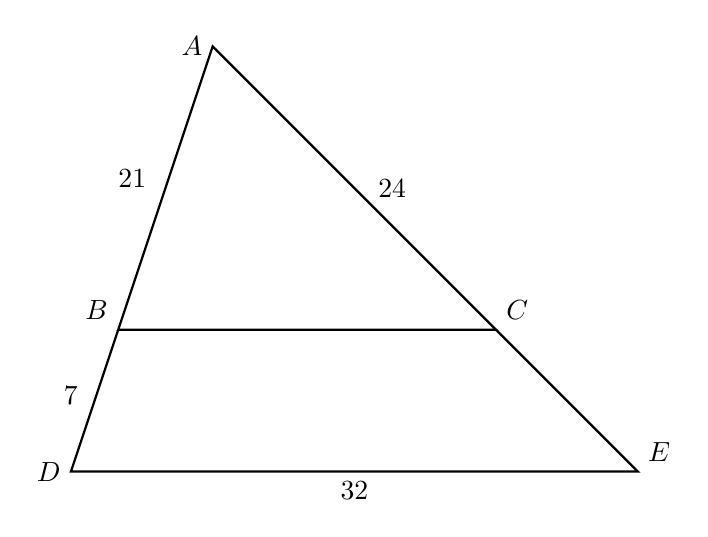
\begin{tikzpicture}[scale=0.6]
    \draw [thick]
    (0,0)node[above left]{$B$}--
    (8,0)node[above right]{$C$}--
    (2,6)node[left]{$A$}--cycle;
    \draw [thick]
    (0,0)--
    (-1,-3)node[left]{$D$}--
    (11,-3)node[above right]{$E$}--(8,0);
    \node at (-1,-1)[below]{$7$};
    \node at (5.3, 3)[right]{$24$};
    \node at (0.3, 2.8)[above]{$21$};
    \node at (5,-3)[below]{$32$};
  \end{tikzpicture}
\end{center}

\newpage
\item Circle $O$ has chords $\overline{AD}$ and $\overline{BE}$ intersecting at $C$, as shown. Find $AC$.
\begin{center}
  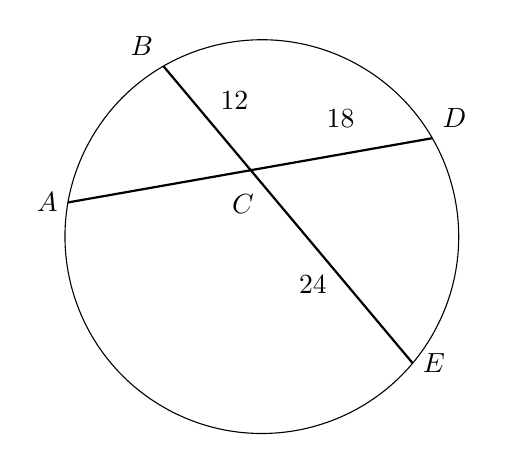
\begin{tikzpicture}[scale=0.5, rotate=-30]
   \draw (0,0) circle[radius=5];
   \draw [thick]
   (-10:5) node[right] {$E$}--
   (150:5) node[above left] {$B$};
   \draw [thick](200:5) node[left] {$A$}--
   (60:5) node[above right] {$D$};
   \draw (140:1.4) node[below] {$C$};
   \draw (130:4) node[below] {$12$};
   \draw (90:4) node[below] {$18$};
   \draw (0:1.5) node[below] {$24$};
  \end{tikzpicture}
\end{center}

\item Point $P$ divides $\overline{AB}$ so that $AP:PB = 1:3$. If $A$ has coordinates $(11,-1)$ and $B$ has coordinates $(-1,7)$, what are the coordinates of $P$?
\vspace{1cm}

\item From six miles away, the angle of elevation to a mountain peak is $11.5^\circ$. What is the height of the mountain above the observer, to the \emph{nearest hundred feet}? (1 mile = 5280 feet)
  \begin{center}
    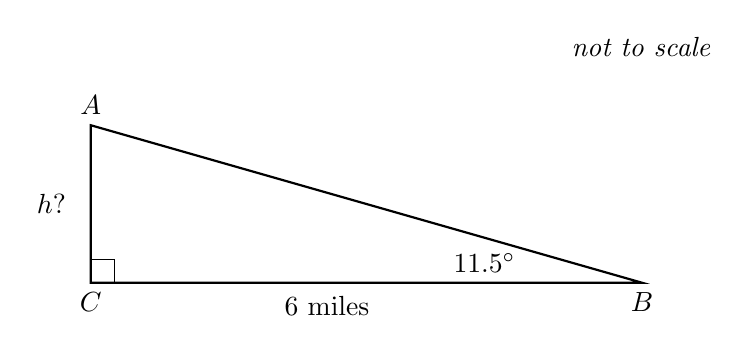
\begin{tikzpicture}[scale=1]
    \draw [thick]
      (0,0)node[below]{$B$}--
      (-7,2)node[above]{$A$}--
      (-7,0)node[below]{$C$}--cycle;
      \draw (-7,0)++(0.3,0)--++(0,0.3)--+(-0.3,0);
      \node at (-7.5,1){$h?$};
      \node at (-2,0.25){$11.5^\circ$};
      \node at (-4,-0.3){6 miles};
      \node at (0,3){\emph{not to scale}};
  \end{tikzpicture}
  \end{center} \vspace{1cm}

\item If a rectangular sheet is continuously rotated around one of its longer edges, what is the three-dimensional figure formed?
  \begin{multicols}{2}
  \begin{enumerate}
    \item cone
    \item sphere
    \item cylinder
    \item rectangular prism
  \end{enumerate}
\end{multicols}

\newpage
\item Rotate the triangle $90^\circ$ clockwise around the origin, $\triangle ABC \rightarrow \triangle A'B'C'$. Plot and label the image on the grid.
  \begin{center}
      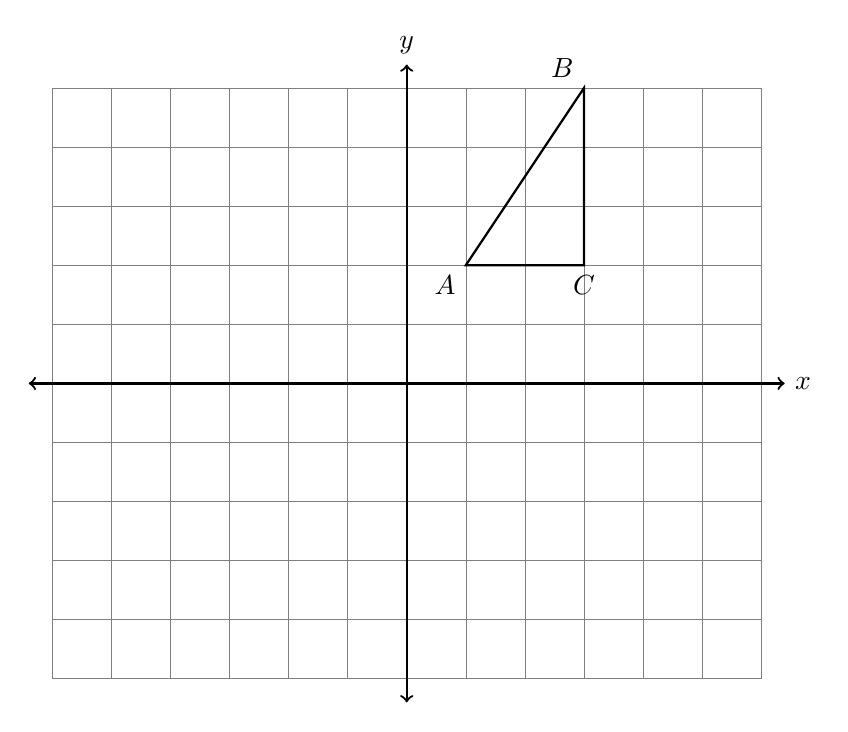
\begin{tikzpicture}[scale=.75]
      \draw [help lines] (-6,-5) grid (6,5);
      \draw [thick, <->] (-6.4,0) -- (6.4,0) node [right] {$x$};
      \draw [thick, <->] (0,-5.4)--(0,5.4) node [above] {$y$};  
      \draw [thick]
        (1,2) node[below left] {$A$}--
        (3,5) node[above left] {$B$}--
        (3,2) node[below] {$C$}--cycle;  
      \end{tikzpicture}
    \end{center}
    
\item What is an equation of the line that passes through the point $(1,-1)$ and is perpendicular to a line with equation $2x-y=5$?
\begin{multicols}{2}
\begin{enumerate}
    \item $y-1=\frac{1}{2}(x+1)$
    \item $y-1=-\frac{1}{2}(x+1)$ 
    \item $y+1=\frac{1}{2}(x-1)$
    \item $y+1=-\frac{1}{2}(x-1)$
\end{enumerate}
\end{multicols}

\item The secants $\overline{ABC}$ and $\overline{ADE}$ intersect the circle $O$, as shown in the diagram. \\Given $m \wideparen{BD}=32^\circ$ and $m \wideparen{CE}=126^\circ$. Find the measure of $\angle A$.
  \begin{center}
  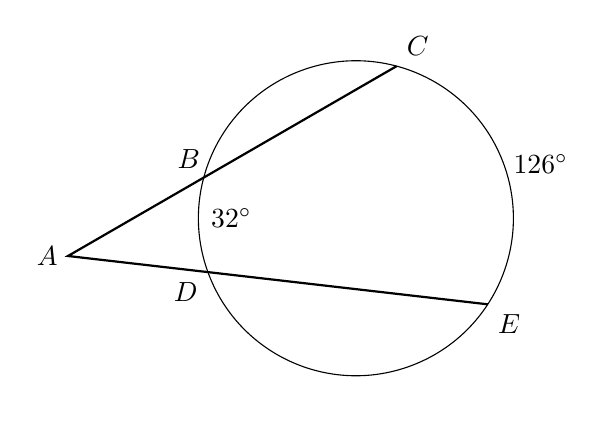
\begin{tikzpicture}[scale=.4, rotate=20]
    \draw (0,0) circle[radius=5];
    \draw [thick]
    (3,-4) node[below right] {$E$}--
    (-5,0) node[below left] {$D$}--
    (-9,2) node[left] {$A$}--
    (55:5) node[above right] {$C$};
    %\draw [thick] (3,-4)--(145:5);
    \draw (138:5) node[left] {$B$};
    \draw (0:5) node[right] {$126^\circ$};
    \draw (160:3) node[left] {$32^\circ$};
  \end{tikzpicture}
  \end{center}

\newpage
\item What is the equation of a circle with center $(3,-5)$ and radius $r=4$?

\item The area of a sector of a circle with diameter measuring 8 cm is $1.60\pi \; \rm{cm}^2$. What is the measure of the central angle that forms the sector?

\item Find $x$ such that for the angles of a right triangle, $\sin (5x + 5)=\cos (25)$.

\item In the diagram below of right triangle $KMI$, altitude $\overline{IG}$ is drawn to hypotenuse $\overline{KM}$. If $KG=6$ and $GM=24$, what is the length of $\overline{IG}$?
\begin{center}
  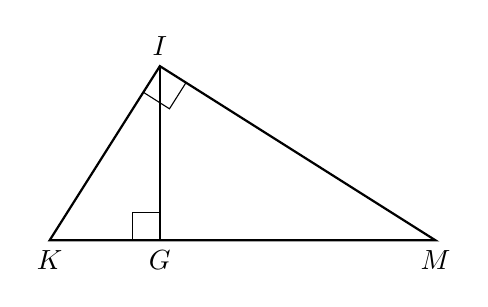
\begin{tikzpicture}[scale=0.7]
  \draw [thick]
  (0,0)node[below]{$K$}--
  (7,0)node[below]{$M$}--
  (2,3.16)node[above]{$I$}--cycle;
  \draw (2,3.16)++(-0.15*2,-0.15*3.16)--++(0.15*3.16,-0.15*2)--+(0.15*2,0.15*3.16);
  \draw [thick](2,0)node[below]{$G$}--(2,3.16);
  \draw (2,0)++(-0.5,0)--++(0,0.5)--+(0.5,0);
\end{tikzpicture}
\end{center}


\item Translate $\triangle DEF$ by $(x,y) \rightarrow (x+3, y+1)$, then reflect the result over the $x$-axis. Label the images $\triangle D'E'F'$ and $\triangle D''E''F''$ respectively.
\begin{center}
    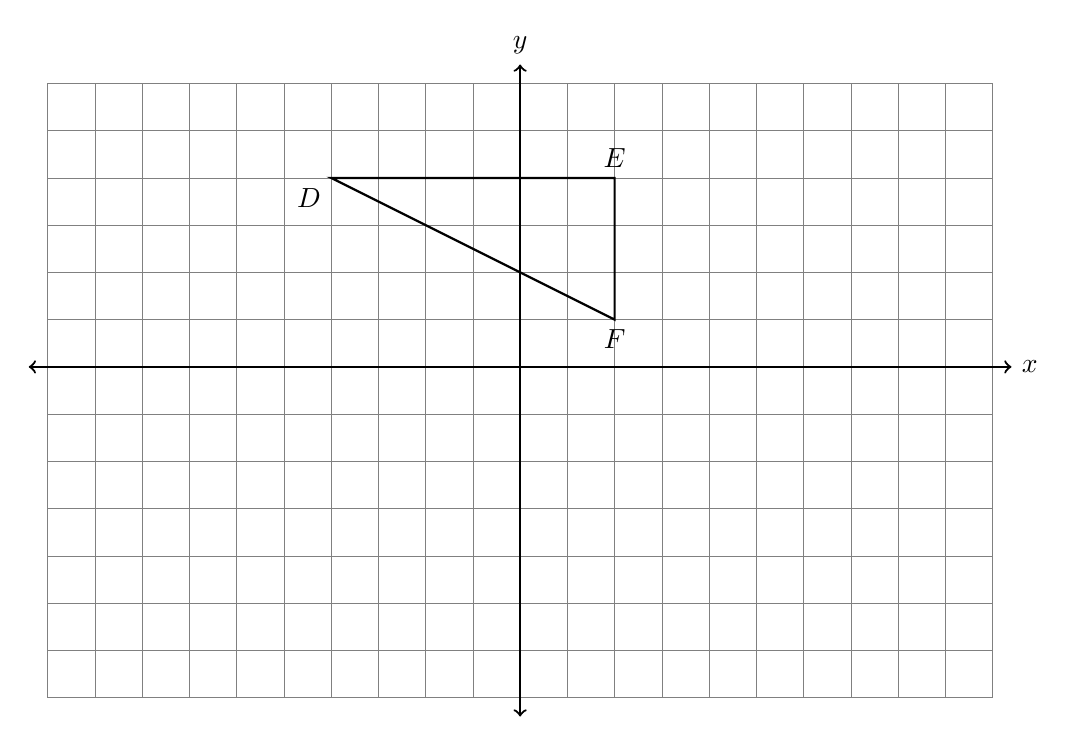
\begin{tikzpicture}[scale=.6]
    \draw [help lines] (-10,-7) grid (10,6);
    \draw [thick, <->] (-10.4,0) -- (10.4,0) node [right] {$x$};
    \draw [thick, <->] (0,-7.4)--(0,6.4) node [above] {$y$};  
    \draw [thick]
      (-4,4) node[below left] {$D$}--
      (2,4) node[above] {$E$}--
      (2,1) node[below] {$F$}--cycle;  
  \end{tikzpicture}
\end{center}

\end{enumerate}
\end{document}
  